\documentclass[11pt,twoside]{article}

%\documentclass{sig-alternate}

\usepackage{jeffe,graphicx,hyperref}
\usepackage[utf8]{inputenc}
\usepackage[margin=1in]{geometry}
\usepackage{marvosym}
\usepackage{cite}
\usepackage{verbatim}

%-----------------------------------------------------------------------
%  These packages are purely cosmetic.
%  Just comment them out if they don't work for you.
%-----------------------------------------------------------------------
\usepackage{microtype}
\usepackage[charter]{mathdesign}
\def\sfdefault{fvs}
\def\ttdefault{fvm}
\usepackage[mathcal]{euscript}
\usepackage{stmaryrd}


%-----------------------------------------------------------------------
%  Local definitions
%-----------------------------------------------------------------------
\def\arcto{\mathord\shortrightarrow}
\def\arc#1#2{#1\arcto#2}
\def\cra#1#2{#1\mathord\shortleftarrow#2}
\def\fence#1#2{#1\mathord\shortuparrow#2}
\def\ecnef#1#2{#1\mathord\shortdownarrow#2}
\def\head{\mathit{head}}
\def\tail{\mathit{tail}}
\def\lsh{\mathit{left}}
\def\rsh{\mathit{right}}
\def\rev{\mathit{rev}}
\def\Z{\mathbb{Z}}
\def\Real{\mathbb{R}}
\def\Q{\mathbb{Q}}

% needs marvosym package:
\def\snip{\mathbin{\raisebox{0.15ex}{\rotatebox[origin=c]{60}{\Rightscissors}\!}}}
\let\unlhd\trianglelefteq	% fix mathdesign font bug

\let\cycle\gamma
\let\path p
\let\primalarc\alpha
\def\dualarc{p}

\def\Sigmabar{\overline{\smash{\Sigma}\vphantom{t}}}
\def\SIGMABAR{\boldsymbol{\overline{\smash{\Sigma}\vphantom{x}}}}
\def\Gbar{\overline{\smash{G}\vphantom{t}}}
\def\Vbar{\overline{\smash{V}\vphantom{t}}}
\def\Ebar{\overline{\smash{E}\vphantom{t}}}
\def\bbar{\overline{\smash{b}\vphantom{t}}}
\def\nbar{\overline{n}}
\def\gbar{\overline{g}}
\def\wbar{\overline{w}}
\def\sigmabar{\overline{\sigma}}
\def\cyclebar{\overline{\cycle}}
\def\chibar{\overline{\chi}}

\def\fakeparagraph#1{\par\medskip\noindent\textbf{#1}}


\newtheorem{theorem}{Theorem}[section]
\newtheorem{corollary}[theorem]{Corollary}
\newtheorem{lemma}[theorem]{Lemma}

\begin{document}

\pagestyle{myheadings}
\markboth{Minimum cuts in surface graphs}
		 {Erin W. Chambers, Jeff Erickson, Kyle Fox, and Amir Nayyeri}

\begin{titlepage}

\title{Minimum cuts in surface graphs\footnote{
Portions of this work done by different subsets of the authors appeared in~\cite{cen-mcshc-09},~\cite{en-mcsnc-11}, and~\cite{efn-gmcse-12}.
}}

\author{
  Erin W. Chambers%
  \thanks{Department of Computer Science and Mathematics, Saint Louis
  University;
  \url{echambe5@slu.edu}.  Supported in part by NSF grants CCF 1054779 and DMS-0528086.
  Portions of this work were done while this author was a student at the University of Illinois at Urbana-Champaign.}
  \and
  Jeff Erickson%
  \thanks{Department of Computer Science,
  University of Illinois, Urbana-Champaign; \url{jeffe@illinois.edu}.
  Supported in part by NSF grants CCF 09-15519 and DMS-0528086.
  }
  \and
  Kyle Fox%
  \thanks{Department of Computer Science,
      University of Illinois, Urbana-Champaign;
      \url{kylefox2@illinois.edu}.
      Supported in part by
      the Department of Energy Office
      of Science Graduate Fellowship Program (DOE SCGF),
      made possible in part by the American Recovery and
      Reinvestment Act of 2009, administered by ORISE-ORAU
      under contract no. DE-AC05-06OR23100.}
  \and
  Amir Nayyeri%
  \thanks{Department of Computer Science,
      Carnegie Mellon University,
      \url{amirn@cs.cmu.edu}. Supported in part by NSF grants
      CCF 1065106, CCF 09-15519, and DMS-0528086. Portions of this work were done while this author was a student 
      at the University of Illinois at Urbana-Champaign.}
      }

\DRAFT

\maketitle
\begin{abstract}
Let $G$ be an edge-weighted directed graph with $n$ vertices embedded on an orientable surface of genus $g$.
We describe algorithms to efficiently compute minimum $s,t$-cuts and global minimum cuts of~$G$.
\note{TODO(kylejfox): Rewrite abstract.}
\end{abstract}

\noindent

\thispagestyle{empty}
\setcounter{page}{0}
\end{titlepage}


%---------------------------------------
\section{Introduction}
\label{sec:intro}

Planar graphs have been a natural focus of study for algorithms research for decades, both because they accurately model many real-world networks, and because they often admit simpler and/or more efficient algorithms for many problems than general graphs.  Most planar-graph algorithms either apply immediately or have been quickly generalized to larger families of graphs, such as graphs of higher genus, graphs with forbidden minors, or graphs with small separators.  Examples include minimum spanning trees \cite{p-omst-99, m-tltam-04}; single-source and multiple-source shortest paths \cite{cc-msspg-07, fr-pgnwe-06, hkrs-fspap-97, k-msspp-05, kmw-spdpg-09, lrt-gnd-79, tm-spltm-09}; graph and subgraph isomorphism \cite{g-itegd-00, hw-ltaip-74, m-itgbg-80, e-sipgr-99, e-dtmcg-00}; and approximation algorithms for the traveling salesman problem, Steiner trees, and other NP-hard problems~\cite{bdt-ptass-08, bkk-ptass-07, bkk-stpg-07, dhm-aacd-07, e-dtmcg-00}.

The classical minimum cut problem and its dual, the maximum flow problem, are stark exceptions to this general pattern.  Flows and cuts were introduced in the 1950s as tools for studying transportation networks, which are naturally modeled as planar graphs \cite{hr-fmern-55}.  Ford and Fulkerson's seminal paper \cite{ff-mfn-56} includes an algorithm to compute maximum flows in planar networks where the source and target lie on the same face.  A long series of results eventually led to planar minimum-cut algorithms that run in $O(n\log n)$ time, first for undirected graphs \cite{r-mstcp-83, hj-oamfu-85, f-faspp-87} and later for directed
graphs \cite{jk-mcdpn-92, hkrs-fspap-97}.
Strangely, however, almost nothing was known about computing flows and cuts in generalizations of planar graphs until very recently~\cite{cen-hfcc-12}.
Even for graphs embedded on the torus, the fastest known minimum-cut algorithms require first computing a maximum flow, a process which takes~$O(n^{3/2})$ time unless edge capacities are sufficiently small integers~\cite{cen-hfcc-12}.

This paper describes the first algorithms to compute minimum cuts in surface-embedded graphs of fixed genus in near-linear time when edges are given real valued capacities.
Two of these algorithms are designed to solve the minimum $(s,t)$-cut problem; the remaining algorithm solves the global minimum cut problem.
Before describing our results in detail, we first review several related results; technical terms are defined in Section \ref{sec:prelims}.

\fakeparagraph{Planar minimum cuts.}
\note{TODO(Kyle): Make sure we do not use ``minimum cut'' when we specifically mean ``minimum $(s,t)$-cut''.}
Recall that for any two vertices $s$ and~$t$ in a graph $G$, an \EMPH{$(s,t)$-cut} is a subset of the edges of $G$ that intersects every path from $s$ to $t$.  A \emph{minimum} $(s,t)$-cut is an $(s,t)$-cut of minimum size, or minimum total weight if the edges of $G$ are weighted.

Itai and Shiloach \cite{is-mfpn-79} observed that the minimum $(s,t)$-cut in a planar graph~$G$ is dual to the minimum-cost cycle that separates faces $s^*$ and $t^*$ in the dual graph $G^*$.  They also observed that this separating cycle intersects any shortest path from a vertex of $s^*$ to a vertex of $t^*$ exactly once.  Thus, one can compute the minimum cut by cutting the dual graph $G^*$ along a shortest path~$\pi$ from $s^*$ to~$t^*$; duplicating every vertex and edge of $\pi$; and then computing, for each vertex $u$ of $\pi$, the shortest path between the two copies of $u$ in the resulting planar graph.  Applying Dijkstra's shortest-path algorithm at each vertex of~$\pi$ immediately yields a running time of $O(n^2\log n)$.

Reif \cite{r-mstcp-83} improved the running time of this algorithm to $O(n\log^2 n)$ using a divide-and-conquer strategy.  Reif's algorithm was extended by Hassin and Johnson to compute the actual maximum flow in $O(n\log n)$ additional time, using a carefully structured dual shortest-path computation \cite{hj-oamfu-85}.  Frederickson~\cite{f-faspp-87} subsequently improved the running time of Reif's algorithm to $O(n\log n)$ using a balanced separator decomposition to speed up the shortest-path computations.  Janiga and Koubek~\cite{jk-mcdpn-92} attempted to adapt Reif's $O(n\log^2 n)$-time algorithm to directed planar graphs\footnote{Unfortunately, their minimum cut algorithm has a subtle
error~\cite{kn-mcupg-11} which may lead to an incorrect result when the
minimum $t,s$-cut is smaller than the minimum $s,t$-cut.}.

Henzinger \etal~\cite{hkrs-fspap-97} generalized Frederickson's technique to obtain an $O(n)$-time planar shortest-path algorithm; using this algorithm in place of Dijkstra's algorithm improves the running times of both Reif's and Janiga and Koubek's algorithms to $O(n\log n)$.  The same improvement can also be obtained using more recent multiple-source shortest path algorithms by Klein~\cite{k-msspp-05} and Cabello and Chambers \cite{cc-msspg-07}.

Minimum $(s,t)$-cuts in directed planar graphs can also be obtained in $O(n\log n)$ time using the planar maximum-flow algorithms of Weihe \cite{w-mstfp-97} (if the graph satisfies certain connectivity restrictions) and Borradaile and Klein \cite{b-epnfc-08, bk-tamfd-06, bk-amfdp-09}.

A \EMPH{cut} (without specified $s$ and $t$) is a subset of edges of $G$ that separate $G$ into two non-empty sets of vertices.
A \emph{minimum} cut is a cut of minimum size, or minimum total weight if the edges of $G$ are weighted.
To differentiate between minimum $(s,t)$-cuts and minimum cuts, we sometimes refer to the latter as global minimum cuts.
Chalermsook, Fakcharoenphol, and Nanongkai~\cite{cfn-dnlta-04} gave the first algorithm for computing global minimum cuts that relies on planarity. Their algorithm runs in~$O(n \log^2 n)$ time. Their algorithm was later improved by \L\c{a}cki and Sankowski~\cite{ls-mcsc-11} who achieved an $O(n \log \log n)$ running time.

\fakeparagraph{Generalizations of planar graphs.}
Surprisingly little is known about the complexity of computing maximum flows or minimum cuts in generalizations of planar graphs.  In particular, we know of no algorithm to compute minimum cuts in non-planar graphs that does not first compute a maximum flow.

By combining a technique of Miller and Naor \cite{mn-fpgms-95} with the planar directed flow algorithm of Borradaile and Klein \cite{b-epnfc-08, bk-tamfd-06, bk-amfdp-09}, one can compute maximum (single-commodity) flows in a planar graph with $k$ sources and sinks in $O(k^2 n\log n)$ time.  A recent algorithm of Hochstein and Weihe \cite{hw-mstfkc-07} computes a maximum flow in a planar graph with $k$ additional edges in $O(k^3n\log n)$ time, using a clever simulation of Goldberg and Tarjan's push-relabel algorithm~\cite{gt-namfp-88}.

Imai and Iwano \cite{ii-espap-90} describe a max-flow algorithm that applies to graphs of positive genus, but not to arbitrary sparse graphs.
Their algorithm computes minimum-cost flows in graphs with small balanced separators, using a combination of nested dissection \cite{lrt-gnd-79, pr-fepss-93}, interior-point methods~\cite{v-slpfm-89}, and fast matrix multiplication.
Their algorithm can be adapted to compute maximum flows (and therefore minimum cuts) in any graph of constant genus in time $O(n^{1.595}\log C)$, where $C$ is the sum of integer edge weights.
However, this algorithm is slower than more recent and more general algorithms \cite{gr-bfdb-98}.
Chambers, Erickson, and Nayyeri~\cite{cen-hfcc-12} describe maximum flow algorithms that are tailored specifically for graphs of constant genus.
Given a graph embedded on a surface of genus~$g$, their algorithms can compute a maximum flow in time $O(g^8 n \log^2 n \log^2 C)$ where $C$ is the sum of integer edge weights and time $g^{O(g)}n^{3/2}$ when edge weights are arbitrary positive real numbers.

Euler's formula implies that a simple $n$-vertex graph embedded on a surface of genus $O(n)$ has at most $O(n)$ edges.
The fastest known combinatorial maximum-flow algorithm for sparse graphs, due to Orlin~\cite{o-mfotl-13}, runs in time $O(n^2 / \log n)$.
The fastest algorithm known for small integer capacities, due to Goldberg and Rao \cite{gr-bfdb-98}, runs in time $O(n^{3/2}\log n\log U)$, where $U$ is an upper bound on the integer edge weights.
Finally, the fastest known algorithm for computing global minimum cuts for sparse graphs, due to Karger~\cite{k-mcnlt-00}, runs in~$O(n \log^3 n)$ time.

For further background on maximum flows, minimum cuts, and related problems, we refer the reader to monographs by Ahuja \etal\ \cite{amo-nftaa-93} and Schrijver \cite{s-cape-03}.

\fakeparagraph{Short interesting cycles.}
Many different problems, such as finding approximate traveling salesman tours  \cite{dhm-aacd-07} and Steiner trees~\cite{bdt-ptass-08} in surface embedded graphs, embedding high-genus graphs into the plane with low distortion \cite{is-pebgg-07} or with few crossings \cite{kr-ccnlt-07}, and feature detection and simplification in meshes \cite{gw-tnr-01,dlsc-cgaht-08}, require algorithms to find short but topologically nontrivial cycles.

Thomassen described the first efficient algorithm to find the shortest non-contractible or non-separating cycle \cite{t-egnsn-90, mt-gs-01}.  After many intermediate improvements \cite{c-mdpg-06, cm-fsnsn-07, eh-ocsd-04, k-csnco-06,cc-msspg-07,insw-iamcmf-11}, Cabello, Chambers, and Erickson~\cite{cce-msspe-13} and Fox~\cite{f-sntcd-13} described the fastest algorithms currently known for this problem, which run in $O(g^2 n \log n)$ and $g^{O(g)} n \log \log n$ time respecitively.
Splitting cycles are non-contractible and separating; finding the shortest such cycle is {NP}-hard, although there is an $O(n \log \log n)$-time algorithm for graphs of any fixed genus \cite{ccelw-scsih-06, ccelw-scsih-08,insw-iamcmf-11}.  Colin de Verdi\`ere and Erickson~\cite{ce-tspcs-06} prove that the shortest path or cycle in a given homotopy class can be computed in polynomial time, improving earlier results of Colin de Verdi\`ere and Lazarus \cite{c-rcds-03, cl-oslos-05, cl-opdsh-07}.  Erickson and Whittlesey describe a greedy algorithm to find a minimum-length set of cycles that generate the first homology group of a surface \cite{ew-gohhg-05}.
\note{TODO:Add references for directed problems too, if only because of the homology cover result.}

Several practical heuristics have been developed for finding short cycles that work well in practice, although they have no theoretical guarantees.  For example, Guskov and Wood \cite{gw-tnr-01} describe an algorithm to find and remove intersecting pairs of short non-contractible cycles (`topological noise') from surface meshes.  Zomorodian and Carlsson \cite{zc-lh-07} define the \emph{localized} homology of an arbitrary topological case with respect to a subspace covering; they also describe algorithms to compute localized homology generators of simplicial complexes using persistent homology; however, they do not describe how to compute covers that would lead to cycles of minimum size.  Chen and Friedman \cite{cf-qhc2-07, cf-qhc-08} describe a polynomial-time algorithm to compute a cycle of minimum \emph{radius} in a given homology class, in an arbitrary edge-weighted simplicial complex; however, the length of this cycle could be arbitrarily longer than optimal.

Dey \etal~\cite{dls-chtl-07, dlsc-cgaht-08} describe algorithms to find short \emph{handle} and \emph{tunnel} cycles in surface meshes embedded in $\Real^3$.  Any embedded surface subdivides $\Real^3$ into an inner handlebody $I$ and an outer handlebody $O$; handle cycles are null-homologous in $I$, while tunnel cycles are null-homologous in~$O$.  The algorithm of Dey \etal\ finds $g$ short handle cycles and $g$ short tunnel cycles that collectively generate the first homology group of the input surface.  Their algorithm uses several heuristics to reduce the length of the output cycles, in part because no algorithm is known to find the shortest cycle in a given homology class.

\subsection{New results and organization}
The input to our first algorithm is an undirected edge-weighted graph~$G$ embedded on an orientable surface of genus~$g$.  Given vertices $s$ and $t$, our algorithm computes a minimum-weight $(s,t)$-cut in $g^{O(g)}n\log \log n$ time.
For any fixed positive genus, this improves the best previous time bound of Chambers, Erickson, and Nayyeri~\cite{cen-hfcc-12} by a factor of $\min\set{ \sqrt{n} / \log \log n, \log^2 n / \log \log n \log^2 C}$ (compared to minimum cut algorithms for general sparse graphs, the improvement is $\min\set{n / ( \log n \log \log n), \sqrt{n} \log n / \log \log n \log C}$).
\note{Mention how this time matches planar algorithm and will be improved when planar improves.}

Our minimum-cut algorithm is a special case of a more general algorithm to compute a minimum-cost \emph{subgraph} in a given $\Z_2$-homology class.  Even when the homology class is specified by a simple cycle, the output representative may be the union of several cycles; see Figure \ref{F:homology2}.  For surfaces with genus $g$ and $b$ boundary components, our algorithm runs in $(g+b)^{O(g+b)}n\log\log n$ time.
We give this algorithm in Section~\ref{sec:crossing}.
In Section~\ref{sec:hardness}, we show that this more general problem is strongly NP-hard, even if the input homology class is specified by a simple cycle; thus, the exponential dependence on the topology of the surface is unavoidable unless {P}={NP}.  We are not aware of any previous algorithmic results for our more general problem.

The input to our second algorithm is a \emph{directed} edge-weighted graph~$G$ embedded on an orientable surface of genus~$g$.
\note{Kyle: Does the surface need to be orientable?}
This algorithm computes a shortest directed \emph{cycle} in a specified $\Z_2$-homology class in $2^{O(g)}n\log n$ time using different techniques from the algorithm above.
We are unaware of any previously published algorithm for this specific problem; however, an algorithm of Chambers \etal~\cite{ccelw-scsih-08} can be modified to find shortest homologous cycles in \emph{undirected} graphs in $g^{O(g)} n\log n \log n$ time.
This problem can be shown to be {NP}-hard, even for undirected graphs, by a reduction from the traveling salesman problem in grid graphs~\cite{ccelw-scsih-08}.
We also show how to extend this algorithm to compute a minimum-weight $(s,t)$-cut in $2^{O(g)}n\log n$ time in an undirected graph.
These algorithms are described in Section~\ref{sec:homcover}.

Our final algorithm takes as input an undirected edge-weighted graph~$G$ embedded on an orientable surface of genus~$g$.
This algorithm computes a minimum-weight cut (global minimum cut) in $g^{O(g)}n\log \log n$ time.
Here, no $s$ or $t$ are specified, our algorithm simply returns a minimum weight subset of edges that separate the vertices of~$G$ into two non-empty sets.
\note{Mention how this time matches planar algorithm and will be improved when planar improves.}
As in the case of computing minimum-weight $(s,t)$-cuts, our algorithm for global minimum cuts depends upon our more general algorithm for minimum-cost subgraphs in given $\Z_2$-homology classes.
As mentioned, the more general problem is NP-hard.

Of course, both versions of the original minimum-cut problem are not NP-hard!
We conjecture that minimum-weight $(s,t)$-cuts and global minimum cuts can be computed in time $O(g^c n\log \log n)$ for some small constant $c$.

As mentioned, Chambers, Erickson, and Nayyeri~\cite{cen-hfcc-12} describe algorithms to compute a maximum flow in surface embedded graphs, using very different techniques from this paper.  Specifically, given a directed graph embedded on an orientable surface of genus~$g$, with two specified vertices $s$ and $t$, they can compute a maximum $(s,t)$-flow in $O(g^8 n\log^2 n\log^2 C)$ time for integer capacities that sum to $C$, or in $g^{O(g)}n^{3/2}$ time for real capacities.  Their key insight is that it suffices to optimize the relative \emph{real} homology class of the flow, rather than directly optimizing the flow itself.

\section{Notation and Terminology}
\label{sec:prelims}

\note{TODO: Write a prelims section.}

\section{Characterizing Homology}
\label{sec:characterizing}

Throughout the paper, we fix a directed graph $G=(V,E)$, a non-negative weight function $w\colon E\to \Real$, and a cellular embedding of $G$ on a surface $\Sigma$ of genus $g$ with $b$ boundaries.
When considering undirected graphs, we assume the weight function is symmetric.
Without loss of generality, we assume that the underlying surface $\Sigma$ has at least one boundary; otherwise, we can remove an arbitrary face of $G$ from~$\Sigma$ without affecting its homology at all.  Let $\delta_1, \dots, \delta_b$ denote the boundary cycles of $\Sigma$, and let $\beta = 2g+b-1$ denote the the first Betti number of $\Sigma$.

In this section, we describe two standard methods for preprocessing a combinatorial surface in~$O(\beta n)$ time, so that the $\Z_2$-homology class of any even subgraph $\eta$ can be computed in $O(\beta)$ time per edge.
Both methods characterize the homology class of any even subgraph using a vector of~$\beta$ bits.
The vectors are computed using a one of two natural generalizations of tree-cotree decompositions~\cite{e-dgteg-03} to surfaces with boundary.
In the first method, the vector is based on the crossings between~$\eta$ and a set of~$\beta$ primal paths.
By carefully selecting these paths, we can place a bound on the number of times a~$\Z_2$-minimal even subgraph can cross any of these paths; this bound is necessary for the algorithm given in Section~\ref{sec:crossing}.
In the second method, the vector is based on the crossings between~$\eta$ and a set of~$\beta$ \emph{dual} paths.
The vectors from the second method are more easily described and computed than the ones in the first, so we opt to use the second method in the algorithm given in Section~\ref{sec:homcover}.



\subsection{Crossing Parity Vectors}

The first method begins by computing a set $P$ of~$\beta$ paths, each of which is the concatenation of two shortest paths (possibly meeting in the interior of an edge), such that the surface $\Sigma\setminus P$ is a topological disk.
Specifically, it constructs a \emph{greedy system of arcs} in $O(\beta n)$ time, using a modification by Chambers \etal~\cite{ccelw-scsih-08} to an algorithm of Erickson and Whittlesey~\cite{ew-gohhg-05} for constructing a \emph{greedy system of loops}.
If the surface has exactly one boundary, then the greedy system of arcs is identical to a greedy system of loops where every loop shares the same basepoint on the boundary.
\note{TODO(kylejfox): Explicitly describe the construction using Henzinger \etal for the shortest paths.}

Let $p_1, p_2, \dots, p_\beta$ denote the paths in $P$.  It is no coincidence that the number of paths in $P$ is equal to the dimension of the homology group $H(G)$.  Indeed, we can identify the homology class of any even subgraph by considering the number of times it crosses each path in $P$, as follows.

For any cycle $\gamma$ and any index $i$, let $x_i(\gamma)$ denote the number of times $\gamma$ crosses the path~$p_i$.  The \EMPH{crossing vector} $x(\gamma)$ is the vector $(x_1(\gamma), \dots, x_\beta(\gamma))$.  The crossing vector of a set of cycles is the sum of the crossing vectors of its elements.
\begin{lemma}
\label{lem:decomposition}
Every even subgraph of an embedded graph has a cycle decomposition.
\end{lemma}

\begin{proof}
Let $H$ be an even subgraph of $G$.  We can decompose $H$ into cycles by specifying, at each vertex $v$, which pairs of incident edges of $H$ are consecutive.  Any pairing that does not create a crossing at $v$ is sufficient.  For example, if $e_1, e_2, \dots, e_{2d}$ are the edges of $H$ incident to $v$, indexed in clockwise order around $v$, we could pair edges $e_{2i-1}$ and $e_{2i}$ for each $i$.  
\end{proof}

Crossing vectors are not well-defined for arbitrary even subgraphs; different cycle decompositions can yield different crossing numbers.  However, the \emph{parity} of the crossing numbers is independent of the cycle decomposition.  The \EMPH{crossing parity vector} of any even subgraph $H$ is the bit vector $\bar{x}(H) = (\bar{x}_1, \dots, \bar{x}_\beta)$, where $\bar{x}_i = 1$ if the path $p_i$ crosses (any cycle decomposition of) $H$ an odd number of times, and $\bar{x}_i = 0$ otherwise.

\begin{lemma}
Two even subgraphs are homologous if and only if their crossing parity vectors are equal.
\end{lemma}

\begin{proof}
Every boundary subgraph is the symmetric difference of facial cycles.  Any non-contractible loop or arc crosses any facial cycle an even number of times; thus, the crossing parity vector of any facial cycle is the zero vector.  Every pair of even subgraphs $H$ and $H'$ satisfies the identity $x(H\oplus H') = x(H) \oplus x(H')$.  Thus, the crossing parity vector of any boundary subgraph is the zero vector.
\end{proof}

\begin{lemma}
We can compute the crossing parity vector of any even subgraph in $O(\beta)$ time per edge after computing~$P$.
\end{lemma}

\begin{proof}
We can compute a cycle decomposition $\gamma_1, \dots, \gamma_r$ of $H$ in $O(1)$ time per edge, by following the proof of Lemma~\ref{lem:decomposition}.
We can compute the number of crossings between any cycle $\gamma_i$ and any path $p_j$ in time proportional to the number of edges in $\gamma_i$.
\end{proof}

\section{Crossing Sequences and Triangulations}
\label{sec:crossing}


Let~$G$ be undirected, and let $H$
be an even subgraph of $G$.  In this section, we describe an
algorithm to compute the minimum-cost even subgraph homologous with
$H$ in $(g+b)^{O(g+b)}n\log n$ time.  In fact, our algorithm can be
modified easily to compute a minimum-cost representative in
\emph{every} homology class in the same asymptotic running time;
there are exactly $2^{2g+\max\set{b-1,0}}$ such classes.
By Lemma~\cite{lem:surface-st-cut}, our algorithm can be used to find a minimum $s,t$-cut in~$G^*$ in the same amount of time.

Our algorithm closely resembles the algorithm of Chambers \etal~\cite{ccelw-scsih-08} for computing a shortest splitting cycle; in fact, our algorithm is somewhat simpler.  The first stage of our algorithm cuts the underlying combinatorial surface into a topological disk by a network of shortest paths as described in Section~\ref{sec:characterizing_crossings}.  Next, we enumerate all possible ways for an even subgraph to intersect each shortest path in the decomposition network $O(g+b)$ times.  We quickly discard any crossing pattern that does not correspond to an even subgraph in the desired homology class.  Each crossing pattern is realized by several \emph{homotopy} classes of sets of non-crossing cycles, which we easily enumerate.  Within each homotopy class, we find a minimum-length set of non-crossing cycles with each crossing pattern using an algorithm of Kutz \cite{k-csnco-06}.  The union of those cycles is an even subgraph in the desired homology class; we return the lightest such subgraph as our output.

\note{TODO(kylejfox): Assume uniqueness of shortest paths in the prelims.}

\subsection{Crossing bound}

Our main technical lemma for this section establishes an upper bound on the number of crossings between an arbitrary shortest path and the minimum-weight even subgraph in any homology class.  Crossing-number arguments were first used by Cabello and Mohar \cite{cm-fsnsn-07} to develop the first subquadratic algorithms for shortest non-contractible and non-separating cycles in undirected surface embedded graphs; their arguments are the foundation of all later improvements of their algorithm \cite{c-mdpg-06, k-csnco-06, cce-msspe-13}.  Our proof is quite similar to the argument of Chambers \etal~\cite{ccelw-scsih-08} that the shortest \emph{splitting} cycle crosses any shortest path $O(g+b)$ times.  However, our new proof is simpler, because the structure we seek is a true subgraph, which need not be connected, rather than a single (weakly) simple closed walk.

As mentioned in Section~\ref{sec:characterizing}, we cannot consistently define when a shortest path crosses an even subgraph.  Instead, we consider the total number of crossings between a shortest path and the cycles in a cycle decomposition.

\begin{lemma}
\label{lem:crossing}
Let $G$ be an edge-weighted graph embedded on a surface with genus $g$ and $b$ boundary components.  Let $H$ be a subgraph of $G$ of minimum weight in its $\Z_2$-homology class, and let $\gamma_1, \gamma_2, \dots, \gamma_r$ be a cycle decomposition of $H$.  The total number of crossings between any shortest path in $G$ and the cycles $\gamma_1, \gamma_2, \dots, \gamma_r$ is at most $6g+2b-3$.
\end{lemma}

\begin{proof}
Let $\sigma(y,z)$ denote the shortest path between any two vertices $y$ and~$z$, and let $\sigma = \sigma(u,v)$ for some vertices $u$ and~$v$.  Uniqueness of shortest paths implies that if $y$ and $z$ are vertices of $\sigma$, either the shortest path $\sigma(y,z)$ or its reversal $\sigma(z,y)$ is a subpath of $\sigma$.  Without loss of generality, we can assume that $\sigma$ crosses each cycle $\gamma_i$ at least once.  For each $i$, let~$x_i$ denote the number of times $\sigma$ and $\gamma_i$ cross, and let $x = x_1 + x_2 + \cdots + x_r$.  We need to prove that $x\le 6g+2b-3$.

Consider the graph $G/\sigma$ obtained from $G$ by contracting $\sigma$ to a single vertex $uv$.  This graph inherits a cellular embedding on $\Sigma$ from the cellular embedding of $G$.  Each cycle $\gamma_i$ is contracted to the union of $x_i$ simple non-crossing loops in $G/\sigma$ with basepoint $uv$.  Altogether, we obtain $x$ loops, which we denote $\ell_1, \ell_2, \dots, \ell_x$.

Suppose some loop $\ell_i$ is contractible.  This loop is the contraction of a path $\pi_i$ in $G$ whose endpoints~$u_i$ and $v_i$ lie in $\sigma$.  The cycle $\delta = \pi_i \cdot \sigma(v_i,u_i)$ is also contractible.  Thus, the even subgraph $H\oplus\delta$ is homologous with $H$.  Moreover, the uniqueness of shortest paths implies that the weight of $H\oplus\delta = H \cup \sigma(v_i,u_i) \setminus \pi_i$ is smaller than the weight of~$H$.  But this contradicts our assumption that $H $ has minimum weight in its homology class.

Now suppose some pair of loops $\ell_i$ and $\ell_j$ are homotopic; by definition, the cycle $\ell_i\cdot\reverse{\ell_j}$ is contractible.  These two loops are contractions of paths $\pi_i$ and $\pi_j$ in $G$ with endpoints in $\sigma$.  Let $u_i$ and~$v_i$ denote the endpoints of $\pi_i$, and let $u_j$ and~$v_j$ denote the endpoints of $\pi_j$.  The cycle $\pi_i \cdot \sigma(v_i,v_j) \cdot \overline{\pi_j} \cdot \sigma(u_j, u_i)$ in $G$ is also contractible.  Let $\delta$ denote the set of edges of $G$ that appear in this cycle exactly once.  If the sub-paths $\sigma(v_i,v_j)$ and $\sigma(u_j, u_i)$ are edge-disjoint, then $\delta$ is a contractible cycle; otherwise, $\delta$ is the union of two non-crossing homotopic cycles.  In either case, $\delta$ is a boundary subgraph, so the symmetric difference $H\oplus\delta$ is homologous with $H$.  Moreover, $H\oplus\delta$ has smaller weight than~$H$, and we obtain another contradiction.

We conclude that the loops $\ell_1, \ell_2, \dots, \ell_x$ lie in distinct nontrivial homotopy classes.  Thus, these loops define an embedding of a single-vertex graph with $x$ edges onto $\Sigma$, where no face of the embedding is a disk bounded by less than three edges.  Euler's formula now implies that $x\le 6g+2b-3$~\cite[Lemma~2.1]{ccelw-scsih-08}.
\end{proof}

We emphasize that different cycle decompositions of the same even subgraph may lead to different numbers of crossings.  Our crossing bound applies to \emph{any} cycle decomposition.
\section{The $\Z_2$-Homology Cover}
\label{sec:homcover}

\note{TODO: Write a section on computing $\Z_2$-minimal cycles and even subgraphs using the SODA 2011 homology covers method.}

\section{NP-Hardness}
\label{sec:hardness}

\note{TODO: Write a section on how computing $\Z_2$-minimal objects is NP-hard.}

\section{Global Minimum Cut}
\label{sec:global}

Let~$G$ be undirected. We now turn our attention computing the global minimum cut of~$G$.
\note{TODO(kylejfox): Don't forget to give background for this problem and its difficulties in the introduction.}
To work with topology in computing a minimum cut, we use the following lemma which is similar very similar to Lemma~\ref{lem:cut-duality}.
We say a null-homologous even subgraph~$\eta$ is a \EMPH{separating subgraph} if it contains at least one edge.

\note{kylejfox: Throughout the dissertation I said vertex sets were cuts. We may need to reconcile with the $s,t$-cut papers.}
\begin{lemma}
\label{lem:mincut-z2}
Let~$G$ be an undirected graph with non-negative edge capacities, cellularly embedded on a surface~$\Sigma$ without boundary, let~$S$ be a minimum cut in~$G$, and let~$C$ be the edges crossing~$S$.  Then~$C^*$ is a minimum weight separating subgraph of~$G^*$.
\end{lemma}

\begin{proof}
  Let~$C$ be the edges crossing an arbitrary cut in~$G$.  The cut partitions the vertices of $G$
  into two disjoint subsets~$S$ and~$T$. Therefore, the dual subgraph~$C^*$
  partitions the faces of~$G^*$ into two disjoint subsets~$S^*$ and~$T^*$.
  Further,~$C^*$ is the boundary of the union of faces in~$S^*$, implying
  that~$C^*$ is null-homologous in~$\Sigma$ and therefore separating.

  Conversely, let~$C^*$ be an arbitrary separating subgraph of~$G^*$.
  As~$C^*$ is null-homologous, it is the boundary of a subset of the faces
  of~$G^*$.  Moreover, because $C^*$ is non-empty, it must be the boundary of
  a \emph{proper, non-empty} subset of faces.  Let $s^*$ and $t^*$ be faces
  of $G^*$ on either side of $C^*$.  Any path from~$s$ to~$t$ in the primal
  graph~$G$ must traverse at least one edge of~$C$.  We conclude that~$C$ crosses
  a cut (in particular, an $s,t$-cut).
\end{proof}

Fix an undirected graph~$G=(V,E)$, a non-negative weight function ${w\colon E\to \Real}$, and a cellular embedding of~$G$ on a surface~$\Sigma$ of genus~$g$ with at least two faces.  In light of Lemma \ref{lem:mincut-z2}, we focus our attention on finding a minimum weight separating subgraph of~$G$. 

Our algorithm separately considers two cases, illustrated in Figure~\ref{fig:global_cases}. Exactly one of these cases must apply to the minimum weight separating subgraph.
\begin{enumerate}
  \item
    Some minimum weight separating subgraph consists of a single contractible simple cycle.
  \item
    Every minimum weight separating subgraph can be decomposed into non-contractible simple cycles.
\end{enumerate}
%
\begin{figure}[h]
\centering
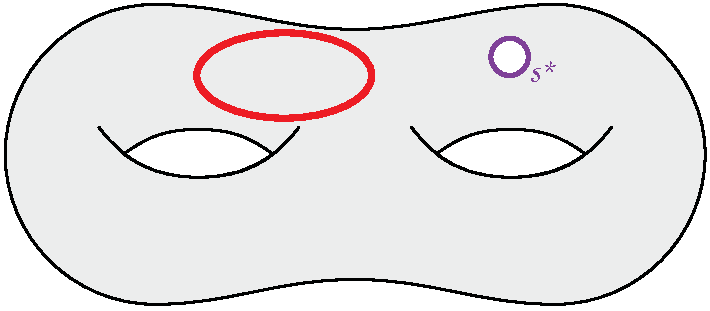
\includegraphics[height=1in]{Fig/shortcon2}\qquad
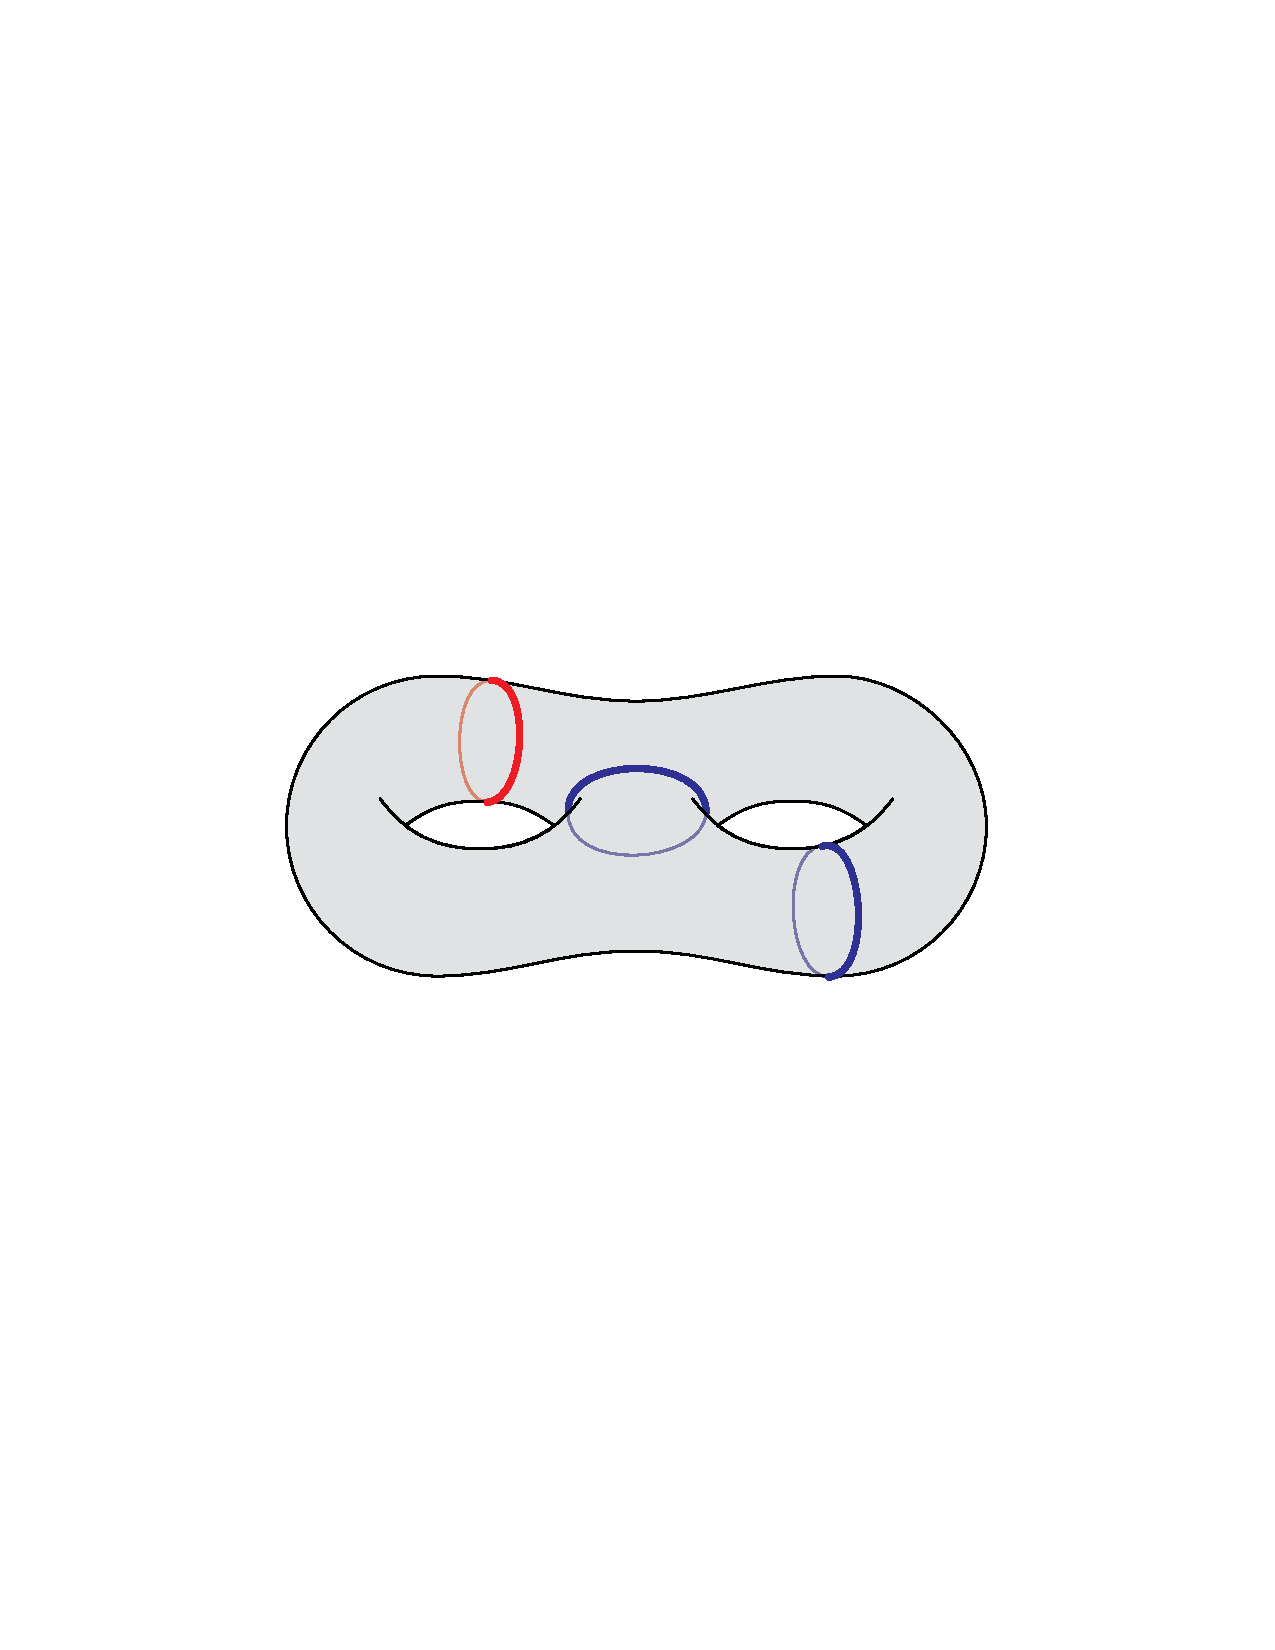
\includegraphics[height=1in]{Fig/homologous1}
\caption{Two types of minimum weight separating subgraphs: a contractible cycle and otherwise.}
\label{fig:global_cases}
\end{figure}
%

Throughout the rest of this section, we describe two subroutines to find minimum weight separating subgraphs that are designed with their corresponding condition in mind. If the corresponding condition does hold, the subroutine will return a separating subgraph with weight at most that of the minimum weight separating subgraph. Otherwise, the subroutine may return a higher weight separating subgraph. By running both subroutines and returning the best result, we find a minimum weight separating subgraph no matter which category it falls into.

\section{Conclusions and Open Problems}

\note{TODO: Write a section on conclusions and open problems.}




% Begin bbl nonsense
\bibliographystyle{abbrv}
\bibliography{topology,data-structures,optimization,other}


\end{document}

